\section{Pre-processing}
My work is focused on the first phase of a data analysis procedure which is the pre-processing.
Data pre-processing (or data preparation) is the process of transforming raw data into a suitable format for modelling. 
Indeed, raw data is in most cases incomplete and noisy.\par
Nowadays, dealing with big amount of information, the probability of incorrect data is higher without a proper data pre-processing.
Only high-quality data can generate accurate models and predictions. \par
Hence, it’s crucial to process data with the best possible quality before training them with artificial intelligence, and machine learning predictive models.\par
For doing this I implemented tools collected in Python Notebooks, each one available in the D-DUST repository:
(\url{https://github.com/opengeolab/D-DUST/tree/thesis_MB}).\newline
Its essential steps (shown in figure \ref{fig:overview}) are these.

\subsection{Data Collection}
Relevant data is gathered from their sources and merged in data structures (such as Dataframes). In our work, data come from fixed ground-sensor, satellite-based platform, models and map layers. In this phase are processed (mostly) numerical and categorical data. 
\subsection{Data Cleaning}
It involves fixing problems or errors in messy or incomplete data. There are general data cleaning operation, such as identifying:
\begin{itemize}
\item duplicate rows of data and remove them;
\item rows with NaN values and remove them;
\item columns that have low variance and drop them;
\end{itemize}
\subsection{Data Transformation}
Data need to be scaled. As a matter of fact, each feature in our data has varying degrees of magnitude, range, and units. This is an issue for machine learning algorithms because of highly sensitive to these features. So in input or output data we performed:
\begin{itemize}
\item Standardization: Scale a feature to a standard Gaussian distribution;
\item Normalization: Scale a feature to the range between 0 and 1;
\end{itemize}
\subsection{Feature Selection}
Feature Selection is the core part of this study. It's the process of reducing the number of input variables when developing a predictive model by basing on a target (or output) variable. 
Data collected, even if have been cleaned and transformed, are anyway characterized by big amount of variables which are redundant.
Discarding irrelevant data is essential before applying Machine Learning model in order to:
\begin{itemize}
\item \textbf{Reduce Overfitting}: less opportunity to make decisions based on noise;
\item \textbf{Improve Accuracy}: less misleading data means that modelling accuracy improves. Predictions can be greatly distorted by redundant attributes;
\item \textbf{Reduce Training Time}: With less data an algorithm will train faster;
\end{itemize}
In this step, which will be explained in detail in the next chapters, the reduced input variables are the ones that are meaningless with respect to a target variable as output. \newline
In this study target variables chosen represent the pollution phenomena such as the PM25 and Ammonia emissions. We choose these targets because are the most relevant sources of pollution produced by intensive agricultural.\newline
One of the aim of this step is to detect main pollutant factors which contribute further on the training of PM25 or NH3 emissions.
Due to the fact that there isn’t a best feature selection technique, many different methods are performed, each one that give different correlation results.\par
After this step, for every method, a score evaluation is assigned to each variable representing its contribution on the output.\par
Finally a voting algorithm is performed in order to average the scores obtained in each feature selection method. 
The highest values are selected for model as input.
\section{Model prediction}
Prediction is a type of analysis that uses techniques and tools to build predictive models and forecast outcomes. In my work predictive analysis is performed for making prediction on pollutants with data processed in the first phase as input.\newline
Model predictions are deployed through regression analysis, used for estimating the relationships between a dependent variable and one or more independent variables.\par
In particular I use supervised techniques based on Machine Learning where the model built is fit with the training dataset and evaluated its performance with the testset. 
\begin{comment}
\begin{itemize}
\item Training data set: //todo  
\item Test data set are made of ground sensor data. In this way the validation is performed with measurement which are most accurate;
\end{itemize}
\end{comment}
For doing prediction, I employ 2 supervised AI models:
\begin{itemize}
\item \textbf{Neural Network regression with Keras}: It's one of the deep learning algorithms that simulate the workings of neurons in the human brain. In a neural network neurons are linked between them forming layers; 
\item \textbf{Machine Learning with Random Forest regressor}: It operates by constructing several decision trees during training time and outputting the mean of the classes as the prediction of all the trees;
\end{itemize}
After this step an evaluation of the performance of predictions is performed in terms of error and accuracy with a procedure called k-fold cross validation.\newline
Finally, a comparison with CAMS data is performed with the aim to demonstrate that the models produced are better estimated in this local scale.\par


\begin{figure}[H]
    \centering
    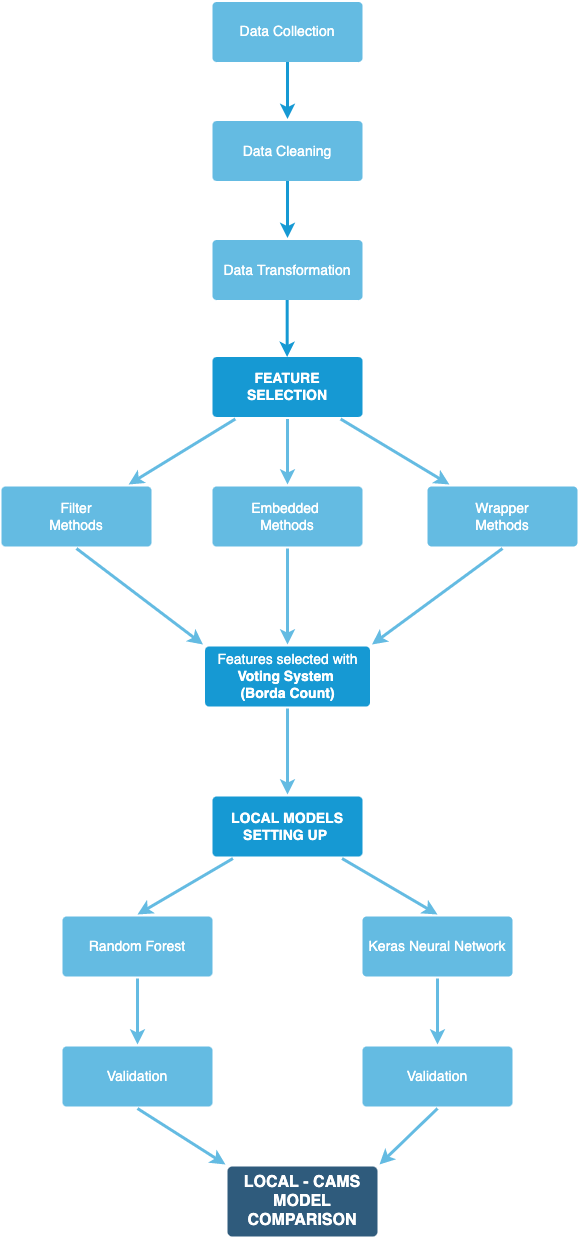
\includegraphics[scale=0.35]{images/overview.png}
    \caption{Overview of the steps made.}
    \label{fig:overview}
\end{figure}

In the next chapters each step will be described in depth about procedures adapted and results obtained.